\documentclass[c]{beamer}
\usepackage{fix-cm}
\usetheme{Berlin}
\usecolortheme{beaver}
\setbeamertemplate{frametitle}[default][center]
\newcommand{\TITLE}{\fontsize{50pt}{1em}\selectfont}
\begin{document}
  \begin{frame}
    \frametitle{}
    \centering
    \textcolor{darkred}{{\TITLE Open Source Licenses}} \\
    \vspace{1em} \hrule \vspace{1em}
    Will Pearson \& Kurt Bruneau
  \end{frame}
  \begin{frame}
    \frametitle{}
    \textcolor{darkred}{{\TITLE Open Source}}
    \vspace{1em} \hrule \vspace{1em}
  \end{frame}
  \begin{frame}
    \frametitle{}
    \textcolor{darkred}{{\TITLE Free Software}} \\
    \vspace{1em} \hrule \vspace{1em}
    \LARGE
    \begin{itemize}
    \item Gratis vs Libre
    \item Four essential freedoms
    \item Copyleft
    \end{itemize}
  \end{frame}
  \begin{frame}
    \frametitle{}
    \textcolor{darkred}{{\TITLE No License?}} \\
  \end{frame}
  \begin{frame}
    \frametitle{}
    \textcolor{darkred}{{\TITLE Do What the Fuck You Want to Public License (WTFPL) \\}}
    Or: Licence Publique Rien À Branler \\
  \end{frame}
  \begin{frame}
    \frametitle{}
    \textcolor{darkred}{{\TITLE MIT \& ISC License \\}}
  \end{frame}
  \begin{frame}
    \frametitle{}
    \textcolor{darkred}{{\TITLE Original BSD License \\}}
    Not actually Open Source. \\
  \end{frame}
  \begin{frame}
    \frametitle{}
    \textcolor{darkred}{{\TITLE Modified \& Simplified BSD Licenses \\}}
    Actually Open Source. \\
  \end{frame}
  \begin{frame}
    \frametitle{}
    \textcolor{darkred}{{\TITLE Apache License v1.0 and v1.1 \\}}
  \end{frame}
  \begin{frame}
    \frametitle{}
    \textcolor{darkred}{{\TITLE Apache License v2.0 \\}}
  \end{frame}
  \begin{frame}
    \frametitle{}
    \textcolor{darkred}{{\TITLE Other Variations \\}}
  \end{frame}
  \begin{frame}
    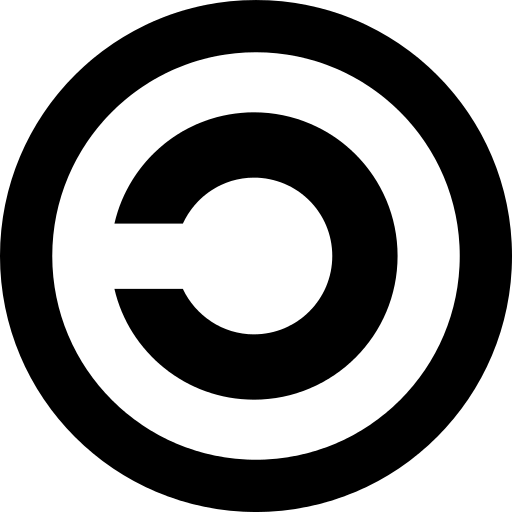
\includegraphics[width=40pt]{copyleft}
    \textcolor{darkred}{{\TITLE opyleft \\}}
    \vspace{1em} \hrule \vspace{1em}
    {\fontsize{20pt}{1em}\selectfont Keep software both open and free}
  \end{frame}
  \begin{frame}
    \textcolor{darkred}{{\TITLE GPLv2}}
    \hfill 
\includegraphics[width=80pt,trim = 0px 150px 0px 0px]{fsf} \\
    \vspace{1em} \hrule \vspace{1em}
    \LARGE
    \begin{itemize}
    \item GNU Linux
    \item Guarantees users freedoms
    \item Most common open source license
    \end{itemize}
  \end{frame}
  \begin{frame}
    \textcolor{darkred}{{\TITLE GPLv3}}
    \hfill 
\includegraphics[width=80pt]{gplv3} \\
    \vspace{1em} \hrule \vspace{1em}
    \LARGE
    \begin{itemize}
    \item GNU Software
    \item Tivoization
    \item DRM
    \item Discriminatory patent deals
     \end{itemize}
  \end{frame}
  \begin{frame}
    \textcolor{darkred}{{\TITLE Other GPL  \\}}
    \vspace{1em} \hrule \vspace{1em}
    \LARGE
    \begin{itemize}
      \item LGPL
      \item AGPL
    \end{itemize}
  \end{frame}

  \begin{frame}
    \textcolor{darkred}{{\TITLE IPL}}
    \hfill 
\includegraphics[width=70pt]{ibm} \\
    \vspace{1em} \hrule \vspace{1em}
    \LARGE
    \begin{itemize}
      \item Derived from GPL
      \item Pushes liabilities to distributors
    \end{itemize}
  \end{frame}

  \begin{frame}
    \textcolor{darkred}{{\TITLE MPL}}
    \hfill 
\includegraphics[width=50pt]{mozilla} \\
    \vspace{1em} \hrule \vspace{1em}
    \LARGE
    \begin{itemize}
    \item Thunderbird, Firefox, Libreoffice
    \item BSD \& GPL Hybrid \\
    \item Buisness \& open source collaboration
    \end{itemize}
  \end{frame}

  \begin{frame}
    \textcolor{darkred}{{\TITLE CDDL}}
    \hfill 
\includegraphics[width=100pt]{sun} \\
    \vspace{1em} \hrule \vspace{1em}
    \LARGE
    \begin{itemize}
    \item Netbeans, Bourne Shell
    \item Derived from MPL
    \end{itemize}
  \end{frame}

  \begin{frame}
    \textcolor{darkred}{{\TITLE APSL}}
    \hfill 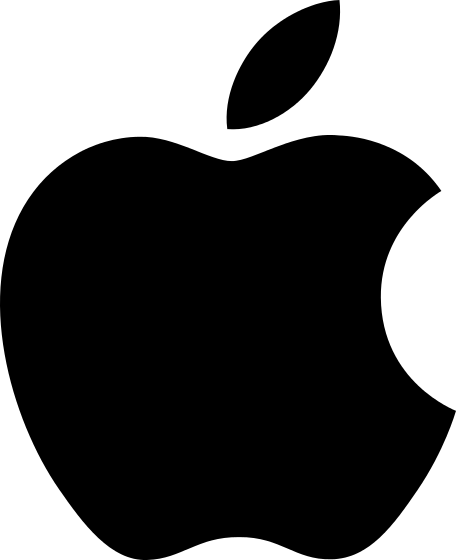
\includegraphics[width=40pt]{apple} \\
    \vspace{1em} \hrule \vspace{1em}
    \LARGE
    \begin{itemize}
    \item Darwin
    \item Not recommended by FSF
    \end{itemize}
  \end{frame}
  \begin{frame}
    \frametitle{}
    \textcolor{darkred}{{\TITLE Choosing and Using a License \\}}
  \end{frame}
  \begin{frame}
    \frametitle{}
    \textcolor{darkred}{{\TITLE Using Other's Software \\}}
  \end{frame}

% etc
\end{document}
